% =====================================================================
%  Fundamentals of Deep Learning — Class 6 (4 August)
%  Topic (course plan): Single-layer NN/Shallow NN
%  Subtopics (course plan): Regression and Classification
%  This class: the classification half.  Regression was Class 5.
%
%  Figures: official vector PDFs from the authors' repositories
%    - Prince figures: github.com/udlbook/udlbook (CC BY-NC-ND)
%    - Bishop figures: authors' published figure set
%  Teaching sequence for Prince figures follows his own Chapter-5
%  lecture slides (CM20315_05_Loss).
%
%  Compile:  xelatex main.tex   (run twice)
% =====================================================================
\documentclass[aspectratio=169, 11pt]{beamer}

\usetheme{metropoliscustom}

\usepackage{graphicx}
\DeclareGraphicsExtensions{.pdf,.png,.jpg}
\graphicspath{{figs_official/}{Class06_Shallow_NN_Classification/A_Textbook_Figures/figs_official/}}
\usepackage{amsmath, amssymb}
\usepackage{bm}
\usepackage{tikz}
\usetikzlibrary{arrows.meta, positioning, calc}
\tcbuselibrary{skins}

\definecolor{mlc}{HTML}{341651}    % ML side (indigo)
\definecolor{nnc}{HTML}{800000}    % NN side (maroon)

% ---- parallel-teaching strip: split box, ML left cell / NN right cell
\newcommand{\mlparallel}[2]{%
  \vfill
  {\footnotesize
  \begin{tcolorbox}[enhanced, sidebyside, sidebyside align=top,
                    lefthand ratio=0.485,
                    segmentation style={mlc!35, line width=0.6pt},
                    colback=mlc!5, colframe=mlc!35, boxrule=0.5pt,
                    arc=1.5mm, left=2mm, right=2mm, top=0.8mm, bottom=0.8mm]
    {\color{mlc}\textbf{ML}}\;\; #1
  \tcblower
    {\color{nnc}\textbf{NN}}\;\; #2
  \end{tcolorbox}}%
  \vspace{0.6em}%
}

% ---- figure source line
\newcommand{\figsource}[1]{{\scriptsize\color{mcMuted} #1}}

% =====================================================================
\title{Single-layer NN/Shallow NN}
\subtitle{Regression and Classification}
\author{Fundamentals of Deep Learning \ \textperiodcentered\ Class 6
        \ \textperiodcentered\ Classification}
\institute{Prof.~Nirav Bhatt}
\date{4 August}

\footleft{Fundamentals of Deep Learning}
\footright{Single-layer NN/Shallow NN}
\titlelogos{}

\begin{document}

\maketitle

\begin{frame}{Outline}
  \tableofcontents
\end{frame}

% =====================================================================
\section{From Regression to Classification}
% =====================================================================

\begin{frame}{What changes}
  \centering
  \renewcommand{\arraystretch}{1.2}
  {\small
  \begin{tabular}{p{0.18\textwidth} p{0.35\textwidth}
                  p{0.35\textwidth}}
    & \textbf{Regression (Class 5)}
    & \textbf{Classification (today)}\\
    \hline
    Target & $t\in\mathbb{R}$
      & $t\in\{0,1\}$ or one of $K$ classes\\
    Output act. & identity
      & \alert{sigmoid} / \alert{softmax}\\
    Loss & sum of squares
      & \alert{cross-entropy}\\
    Prediction & a value
      & a \alert{probability}\\
    \hline
  \end{tabular}}
  \vspace{0.5em}

  {\small The hidden layer is \alert{unchanged}: same
  architecture, same learned features $z_j=h(a_j)$.}
  \mlparallel{linear regression $\to$ logistic regression}
             {NN regression $\to$ NN classification ---
              same translation}
\end{frame}

\begin{frame}{Recap: the shallow network}
  From Class~5 (Bishop \& Bishop, 2024, Eqs.~6.1--6.3):
  \[
    a_j = \sum_{i} w_{ji}^{(1)} x_i + w_{j0}^{(1)},
    \qquad
    z_j = h(a_j),
    \qquad
    a_k = \sum_{j} w_{kj}^{(2)} z_j + w_{k0}^{(2)}
  \]
  \vspace{-0.2em}
  \begin{itemize}\setlength{\itemsep}{1pt}
    \item Regression: $y_k = a_k$ --- the output
          \emph{is} the pre-activation
    \item Classification: pass $a_k$ through an
          \alert{output activation} that produces a
          probability
    \item Everything before the output activation is
          identical
  \end{itemize}
  \mlparallel{$\mathbf{w}^{\!\top}
              \boldsymbol{\phi}(\mathbf{x})$, then
              squash}
             {$\sum_j w_{kj}^{(2)}z_j + w_{k0}^{(2)}$,
              then squash --- features learned}
\end{frame}

% =====================================================================
\section{Linear Classifiers and Decision Boundaries}
% =====================================================================

\begin{frame}{Discriminant functions}
  \begin{columns}[T, onlytextwidth]
    \begin{column}{0.5\textwidth}
      {\small The simplest classifier
      (Bishop \& Bishop, 2024, \S5.1.1):}
      \[
        y(\mathbf{x}) = \mathbf{w}^{\!\top}\mathbf{x}
        + w_0
      \]
      \begin{itemize}\setlength{\itemsep}{1pt}
        \item Assign $\mathcal{C}_1$ if
              $y(\mathbf{x})\ge 0$, else $\mathcal{C}_2$
        \item Boundary $y(\mathbf{x})=0$: a hyperplane
              with normal $\mathbf{w}$, offset set by
              $w_0$
      \end{itemize}
    \end{column}
    \hfill
    \begin{column}{0.46\textwidth}
      \centering
      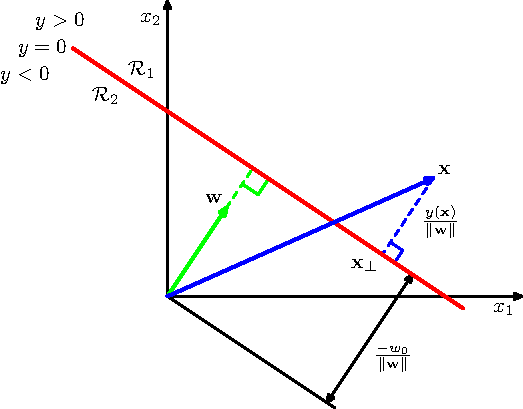
\includegraphics[width=0.66\linewidth]{Bishop5_1}
      \\[0.1em]
      \figsource{Bishop \& Bishop (2024), Fig.~5.1.}
    \end{column}
  \end{columns}
  \mlparallel{decision boundary: a hyperplane in input
              space}
             {a hyperplane in \emph{learned feature}
              space --- nonlinear in $\mathbf{x}$}
\end{frame}

\begin{frame}{Why not just do least squares?}
  \begin{columns}[T, onlytextwidth]
    \begin{column}{0.47\textwidth}
      \centering
      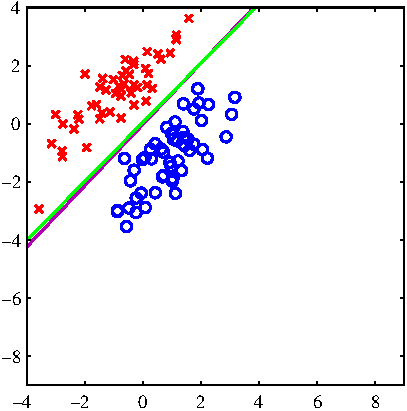
\includegraphics[height=0.40\textheight]{Bishop5_4a}
    \end{column}
    \hfill
    \begin{column}{0.47\textwidth}
      \centering
      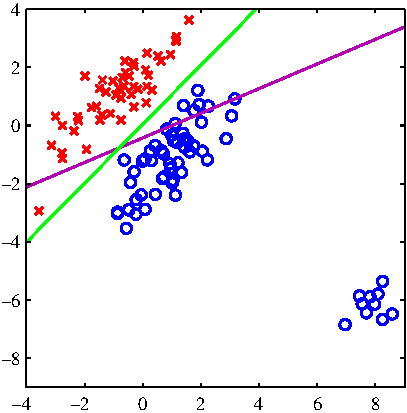
\includegraphics[height=0.40\textheight]{Bishop5_4b}
    \end{column}
  \end{columns}
  \vspace{0.2em}
  \centering
  \figsource{Bishop \& Bishop (2024), Fig.~5.4:
  least squares (magenta) vs.\ logistic regression
  (green).}
  \vspace{0.3em}
  \begin{itemize}\setlength{\itemsep}{1pt}
    \item Adding distant, \emph{correctly classified}
          points drags the least-squares boundary ---
          they are penalised for being ``too right''
    \item Squared error is the wrong loss for targets in
          $\{0,1\}$: we need a loss built for
          \alert{probabilities}
  \end{itemize}
\end{frame}

\begin{frame}{Where the sigmoid comes from}
  \begin{columns}[T, onlytextwidth]
    \begin{column}{0.47\textwidth}
      \centering
      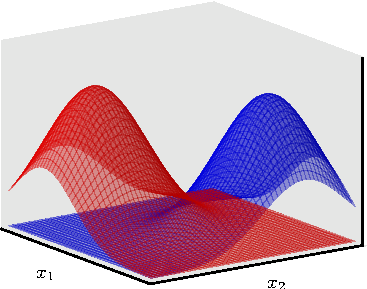
\includegraphics[height=0.34\textheight]{Bishop5_13a}
      \\[0.1em]
      \figsource{class-conditionals
      $p(\mathbf{x}\mid\mathcal{C}_k)$ ---
      B\&B (2024), Fig.~5.13}
    \end{column}
    \hfill
    \begin{column}{0.47\textwidth}
      \centering
      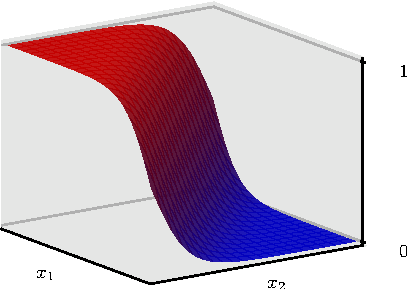
\includegraphics[height=0.34\textheight]{Bishop5_13b}
      \\[0.1em]
      \figsource{posterior
      $p(\mathcal{C}_1\mid\mathbf{x})$ --- a sigmoid}
    \end{column}
  \end{columns}
  \vspace{0.2em}
  \begin{itemize}\setlength{\itemsep}{1pt}
    \item Gaussian classes, shared covariance
          $\Rightarrow$ posterior is \alert{exactly}
          $\sigma(\mathbf{w}^{\!\top}\mathbf{x}+w_0)$
          \hfill{\scriptsize Bishop \& Bishop, \S5.3}
    \item The sigmoid is the \alert{natural form of a
          posterior probability}, not an arbitrary
          squashing choice
  \end{itemize}
\end{frame}

% =====================================================================
\section{The Maximum-Likelihood Recipe}
% =====================================================================

\begin{frame}{The recipe for a loss function}
  The network predicts, for each input, the
  \alert{parameters of a probability distribution} over
  the output (Prince, 2023, \S5.1--5.2):
  \vspace{0.2em}
  \begin{enumerate}\setlength{\itemsep}{2pt}
    \item Choose a distribution
          $Pr(y\mid\bm\theta)$ suited to the
          \alert{domain of $y$}
    \item Let the network predict its parameters:
          $\bm\theta = \mathrm{f}[x,\bm\phi]$
    \item Train by minimising the
          \alert{negative log-likelihood}:
  \end{enumerate}
  \[
    \hat{\bm\phi} = \operatorname*{argmin}_{\bm\phi}
    \Big[-\sum_{i}
    \log Pr\big(y_i \mid \mathrm{f}[x_i,\bm\phi]\big)
    \Big]
  \]
  \begin{itemize}\setlength{\itemsep}{1pt}
    \item Log: products of small numbers $\to$ sums;
          same maximum (log is monotonic)
    \item Inference: report the \alert{peak} of the
          predicted distribution
  \end{itemize}
\end{frame}

\begin{frame}{You already know one instance}
  \begin{columns}[T, onlytextwidth]
    \begin{column}{0.55\textwidth}
      \centering
      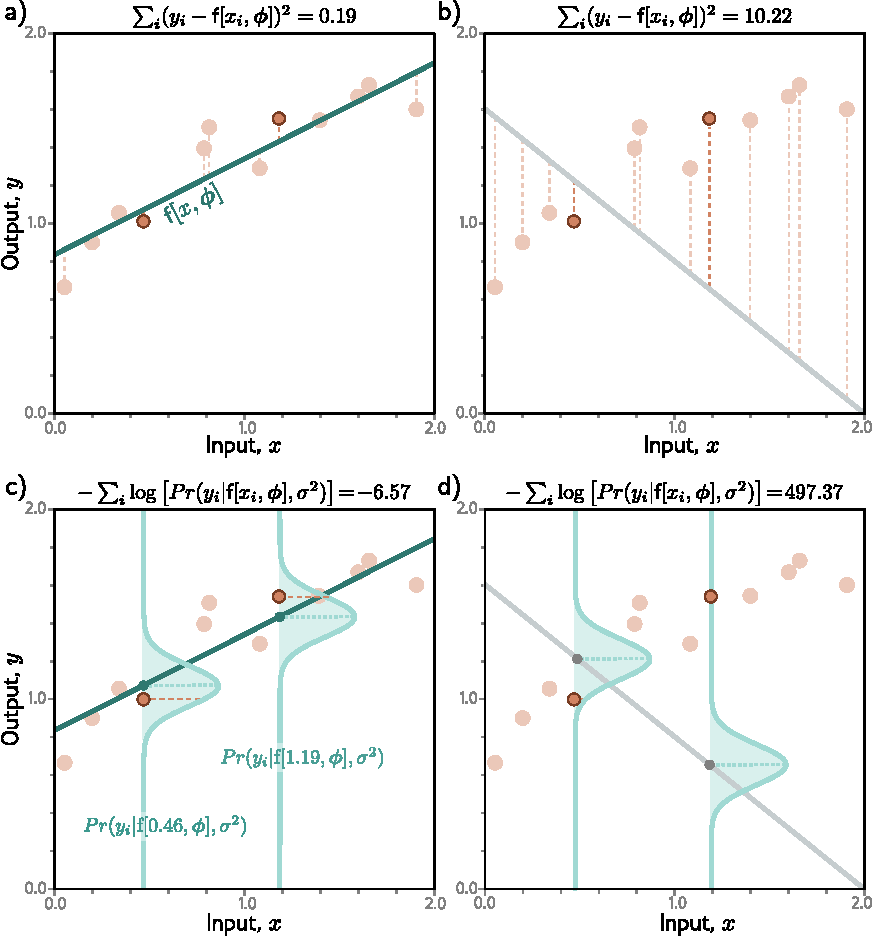
\includegraphics[height=0.48\textheight]{LossNormalRegression}
      \\[0.1em]
      \figsource{Prince (2023), Fig.~5.4.}
    \end{column}
    \hfill
    \begin{column}{0.41\textwidth}
      \vspace{0.2em}
      {\small Class 5, rewritten as the recipe:}
      \begin{itemize}\setlength{\itemsep}{2pt}
        \item {\small Domain $y\in\mathbb{R}$ $\to$
              choose a \alert{Gaussian}}
        \item {\small Network predicts its mean
              $\mu = \mathrm{f}[x,\bm\phi]$}
        \item {\small Negative log-likelihood
              $=$ \alert{least squares}}
      \end{itemize}
    \end{column}
  \end{columns}
  \mlparallel{Gaussian noise $\to$ squared error
              (B\&B \S4.1.1)}
             {today: Bernoulli $\to$ cross-entropy,
              same recipe}
\end{frame}

% =====================================================================
\section{Binary Classification}
% =====================================================================

\begin{frame}{Step 1: the Bernoulli distribution}
  \begin{columns}[T, onlytextwidth]
    \begin{column}{0.5\textwidth}
      {\small Domain: $y\in\{0,1\}$. One parameter
      $\lambda\in[0,1]$:}
      \[
        Pr(y\mid\lambda)
        = \lambda^{y}\,(1-\lambda)^{1-y}
      \]
      \begin{itemize}\setlength{\itemsep}{2pt}
        \item $Pr(y{=}1)=\lambda$, \;
              $Pr(y{=}0)=1-\lambda$
        \item The network must predict
              $\lambda$ --- a number in $[0,1]$
        \item But network outputs are
              \alert{arbitrary real values}\dots
      \end{itemize}
    \end{column}
    \hfill
    \begin{column}{0.44\textwidth}
      \centering
      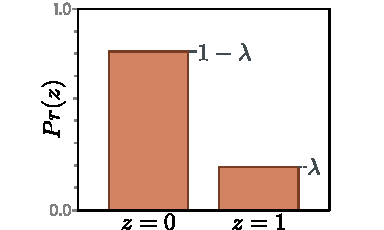
\includegraphics[width=0.7\linewidth]{LossBern}
      \\[0.1em]
      \figsource{Prince (2023), Fig.~5.6.}
    \end{column}
  \end{columns}
\end{frame}

\begin{frame}{Step 2: the logistic sigmoid}
  \begin{columns}[T, onlytextwidth]
    \begin{column}{0.52\textwidth}
      {\small Map the real line to $[0,1]$
      (Bishop \& Bishop, 2024, Eq.~5.42):}
      \[
        \sigma(a) = \frac{1}{1+\exp(-a)}
      \]
      \vspace{-0.5em}
      \begin{itemize}\setlength{\itemsep}{1pt}
        \item $\sigma(0)=\tfrac12$; \;
              symmetry $\sigma(-a)=1-\sigma(a)$
        \item Derivative
              $\sigma'(a)=\sigma(a)(1{-}\sigma(a))$
              \hfill{\scriptsize Eq.~5.72}
        \item So: $\lambda
              = \sigma\big(\mathrm{f}[x,\bm\phi]\big)$
              --- a valid probability
      \end{itemize}
    \end{column}
    \hfill
    \begin{column}{0.42\textwidth}
      \centering
      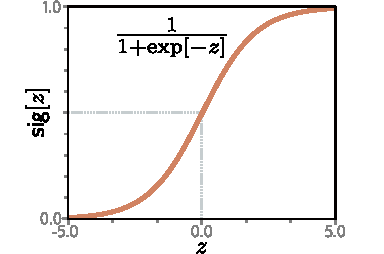
\includegraphics[width=0.72\linewidth]{LossLogisticSigmoid}
      \\[0.1em]
      \figsource{Prince (2023), Fig.~5.7.}
    \end{column}
  \end{columns}
  \mlparallel{logistic regression:
              $\sigma(\mathbf{w}^{\!\top}
              \boldsymbol{\phi}(\mathbf{x}))$}
             {same sigmoid on a \emph{learned-feature}
              read-out}
\end{frame}

\begin{frame}{The binary classification model}
  \centering
  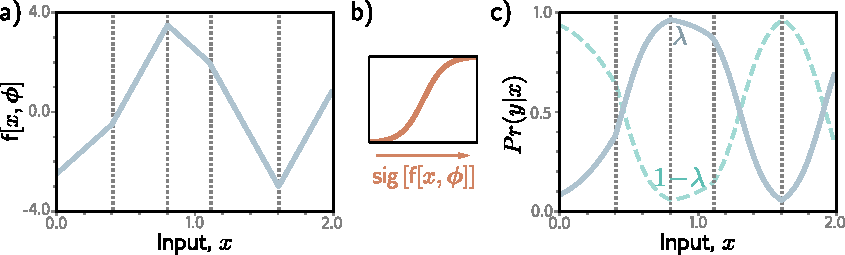
\includegraphics[width=0.76\linewidth]{LossBinaryClassification}
  \\[0.1em]
  \figsource{Prince (2023), Fig.~5.8: (a)~network output;
  (b)~after the sigmoid: probability $\lambda(x)$;
  (c)~likelihood per point.}
\end{frame}

\begin{frame}{Step 3: binary cross-entropy}
  Negative log-likelihood of the Bernoulli model, with
  $y_n=\sigma(a_n)$ read as
  $p(t_n{=}1\mid\mathbf{x}_n)$
  (Bishop \& Bishop, 2024, Eq.~5.74):
  \[
    E(\mathbf{w}) = -\sum_{n=1}^{N}\Big[
      t_n\ln y_n + (1-t_n)\ln(1-y_n)\Big]
  \]
  \vspace{-0.5em}
  \begin{itemize}\setlength{\itemsep}{0pt}
    \item $t_n{=}1$ penalises small $y_n$; \
          $t_n{=}0$ penalises large $y_n$
    \item Gradient (Eq.~5.75):
          $\nabla E = \sum_n (y_n - t_n)\,
          \boldsymbol{\phi}_n$ --- the
          \alert{same $y-t$ form} as least squares
    \item Non-convex with a network inside; convex in
          the output layer alone
  \end{itemize}
  \mlparallel{logistic regression: cross-entropy,
              convex}
             {same loss; non-convex in all parameters}
\end{frame}

\begin{frame}{Why not squared error on probabilities?}
  With a sigmoid output and squared error:
  \[
    \frac{\partial E_{\mathrm{SSE}}}{\partial a_n}
    = (y_n - t_n)\,\sigma'(a_n),
    \qquad
    \frac{\partial E_{\mathrm{CE}}}{\partial a_n}
    = y_n - t_n
  \]
  \vspace{-0.2em}
  \begin{itemize}\setlength{\itemsep}{1pt}
    \item Saturated output ($y_n\!\approx\!0$ or $1$):
          $\sigma'(a_n)\approx 0$ $\to$ the SSE
          \alert{gradient vanishes} even when the
          prediction is wrong
    \item Cross-entropy has no $\sigma'$ factor ---
          learning does not stall
    \item This is the recipe at work: \alert{match the
          loss to the output distribution}
  \end{itemize}
  \vspace{0.3em}
  \begin{redhighlight}
    Distribution $\to$ loss. Gaussian $\to$ squared
    error; Bernoulli $\to$ cross-entropy.
  \end{redhighlight}
\end{frame}

% =====================================================================
\section{Multi-class Classification}
% =====================================================================

\begin{frame}{Step 1: the categorical distribution}
  \begin{columns}[T, onlytextwidth]
    \begin{column}{0.5\textwidth}
      {\small Domain: $y\in\{1,\dots,K\}$. Parameters
      $\lambda_1,\dots,\lambda_K$:}
      \[
        Pr(y{=}k) = \lambda_k,
        \qquad
        \lambda_k \ge 0,\;\;
        \textstyle\sum_k \lambda_k = 1
      \]
      \begin{itemize}\setlength{\itemsep}{2pt}
        \item The network must predict $K$ numbers
              that are positive and sum to one
        \item $K$ raw outputs $a_1,\dots,a_K$ are
              unconstrained\dots
      \end{itemize}
    \end{column}
    \hfill
    \begin{column}{0.44\textwidth}
      \centering
      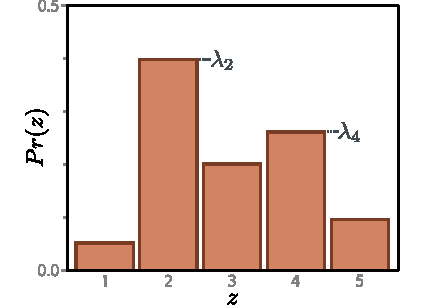
\includegraphics[width=0.72\linewidth]{LossCategorical}
      \\[0.1em]
      \figsource{Prince (2023), Fig.~5.9.}
    \end{column}
  \end{columns}
\end{frame}

\begin{frame}{Step 2: softmax}
  Normalise the $K$ pre-activations
  (Bishop \& Bishop, 2024, Eqs.~5.76--5.77):
  \[
    y_k = \mathrm{softmax}_k(\mathbf{a})
    = \frac{\exp(a_k)}{\sum_{j=1}^{K}\exp(a_j)}
  \]
  \vspace{-0.3em}
  \begin{itemize}\setlength{\itemsep}{1pt}
    \item $y_k>0$ and $\sum_k y_k = 1$ --- a valid
          categorical parameter vector
    \item $K{=}2$ recovers the sigmoid:
          $\mathrm{softmax}$ on $(a_1,a_2)$
          $=\sigma(a_1{-}a_2)$
    \item Adding a constant to every $a_k$ changes
          nothing (used for numerical stability)
  \end{itemize}
  \mlparallel{multinomial (softmax) logistic
              regression}
             {softmax on $K$ learned-feature read-outs}
\end{frame}

\begin{frame}{Softmax posteriors, visualised}
  \begin{columns}[T, onlytextwidth]
    \begin{column}{0.47\textwidth}
      \centering
      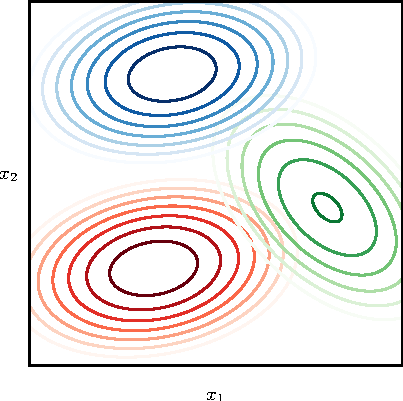
\includegraphics[height=0.38\textheight]{Bishop5_14a}
      \\[0.1em]
      \figsource{three Gaussian classes}
    \end{column}
    \hfill
    \begin{column}{0.47\textwidth}
      \centering
      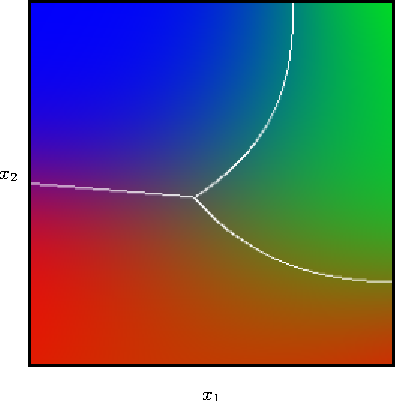
\includegraphics[height=0.38\textheight]{Bishop5_14b}
      \\[0.1em]
      \figsource{posterior class probabilities (RGB)}
    \end{column}
  \end{columns}
  \vspace{0.2em}
  \centering
  \figsource{Bishop \& Bishop (2024), Fig.~5.14.}
  \vspace{0.3em}
  \begin{itemize}\setlength{\itemsep}{1pt}
    \item Softmax posteriors partition input space;
          colours blend where classes overlap
    \item Decision boundaries: where the largest two
          posteriors are equal
  \end{itemize}
\end{frame}

\begin{frame}{The multi-class model}
  \centering
  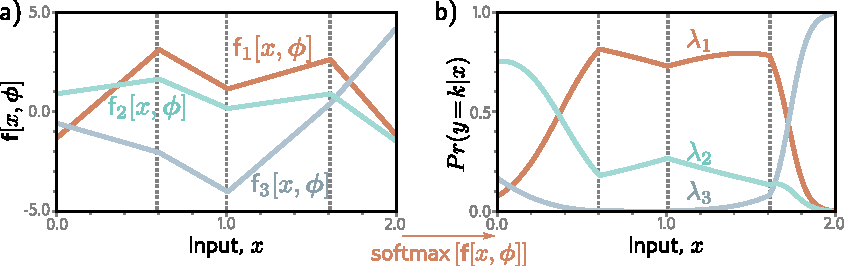
\includegraphics[width=0.88\linewidth]{LossMultiClassClassification}
  \\[0.1em]
  \figsource{Prince (2023), Fig.~5.10 ($K{=}3$):
  (a)~three piecewise-linear outputs; (b)~after softmax
  --- non-negative, sum to one; (c)~decision regions.
  Shared hidden units $\Rightarrow$ joints in the same
  places.}
\end{frame}

\begin{frame}{Step 3: multi-class cross-entropy}
  One-hot targets $\mathbf{t}_n\in\{0,1\}^K$,
  $\sum_k t_{nk}=1$
  (Bishop \& Bishop, 2024, Eq.~5.80):
  \[
    E(\mathbf{w}) = -\sum_{n=1}^{N}\sum_{k=1}^{K}
    t_{nk}\,\ln y_{nk}
  \]
  \vspace{-0.3em}
  \begin{itemize}\setlength{\itemsep}{1pt}
    \item Only the true class contributes: maximise the
          log-probability the model assigns to it
    \item Gradient (Eq.~5.81):
          $\partial E/\partial a_{nk} = y_{nk}-t_{nk}$
          --- \alert{$y-t$ again}
    \item Reduces to binary cross-entropy for $K{=}2$
  \end{itemize}
  \mlparallel{softmax regression: convex in
              $\mathbf{w}$}
             {network inside: non-convex, trained by
              gradient descent}
\end{frame}

% =====================================================================
\section{The Bigger Picture}
% =====================================================================

\begin{frame}{One recipe, any output type}
  \centering
  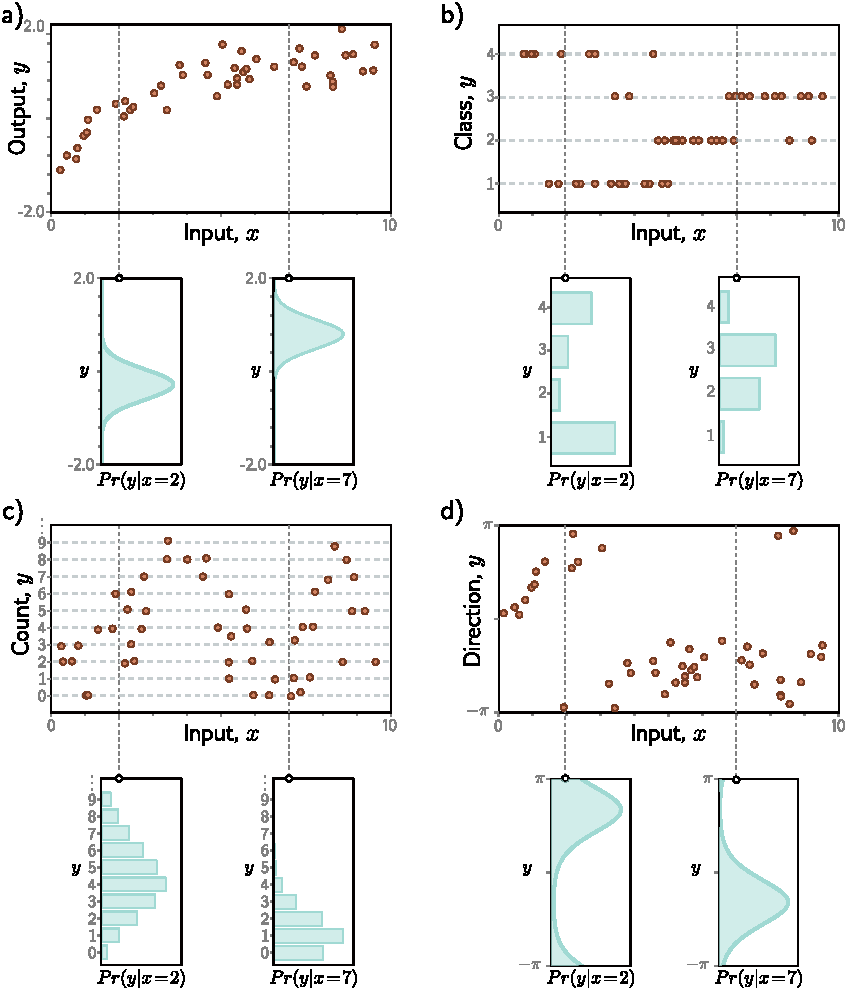
\includegraphics[height=0.62\textheight]{LossDataTypes}
  \\[0.1em]
  \figsource{Prince (2023), Fig.~5.11: choose the
  distribution to match the prediction domain ---
  univariate/multivariate, continuous/discrete, circular,
  bounded, count data.}
\end{frame}

\begin{frame}{Cross-entropy: the second view}
  \begin{columns}[T, onlytextwidth]
    \begin{column}{0.56\textwidth}
      \centering
      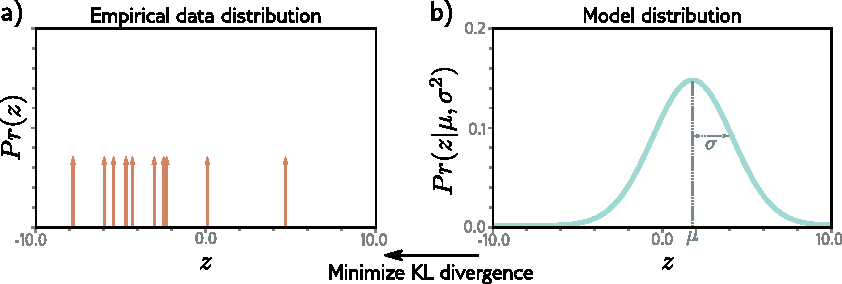
\includegraphics[width=\linewidth]{LossCrossEntropy}
      \\[0.1em]
      \figsource{Prince (2023), Fig.~5.12.}
    \end{column}
    \hfill
    \begin{column}{0.40\textwidth}
      \vspace{0.2em}
      \begin{itemize}\setlength{\itemsep}{2pt}
        \item {\small Minimising negative
              log-likelihood $\equiv$ minimising the
              \alert{KL divergence} between the
              empirical data distribution and the
              model distribution}
        \item {\small The remaining term is the
              \alert{cross-entropy} --- hence the
              loss's name
              \hfill{\scriptsize Prince, \S5.7}}
      \end{itemize}
    \end{column}
  \end{columns}
\end{frame}

\begin{frame}{Fixed features vs.\ learned features, again}
  \begin{columns}[T, onlytextwidth]
    \begin{column}{0.47\textwidth}
      \centering
      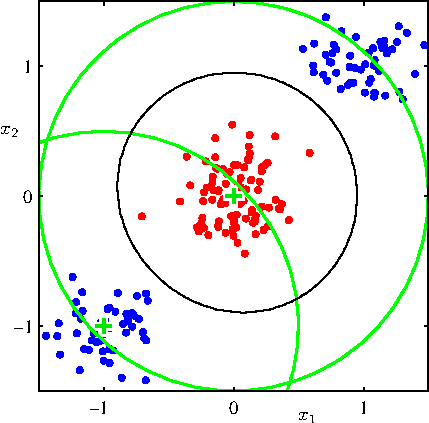
\includegraphics[height=0.38\textheight]{Bishop5_15a}
      \\[0.1em]
      \figsource{input space: nonlinear boundary}
    \end{column}
    \hfill
    \begin{column}{0.47\textwidth}
      \centering
      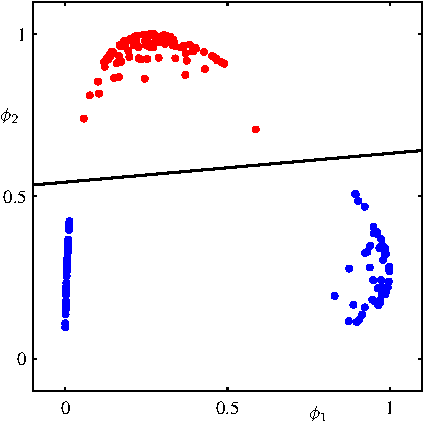
\includegraphics[height=0.38\textheight]{Bishop5_15b}
      \\[0.1em]
      \figsource{feature space
      $(\phi_1,\phi_2)$: linear boundary}
    \end{column}
  \end{columns}
  \vspace{0.15em}
  \centering
  \figsource{Bishop \& Bishop (2024), Fig.~5.15;
  cf.\ Fig.~5.16 for the network view.}
  \mlparallel{fixed Gaussian $\boldsymbol{\phi}$
              linearise the problem}
             {a shallow network \emph{learns} the
              features that linearise it}
\end{frame}

\begin{frame}{Output activations: the complete table}
  \centering
  \renewcommand{\arraystretch}{1.2}
  {\small
  \begin{tabular}{p{0.15\textwidth} p{0.15\textwidth}
                  p{0.24\textwidth} p{0.30\textwidth}}
    \textbf{Task} & \textbf{Distribution} &
    \textbf{Output activation} & \textbf{Loss}\\
    \hline
    Regression & Gaussian &
      identity &
      sum of squares\\
    Binary cl. & Bernoulli &
      sigmoid $\sigma(a)$ &
      binary cross-entropy\\
    Multi-class & categorical &
      softmax &
      cross-entropy\\
    \hline
  \end{tabular}}
  \vspace{0.5em}

  {\small In all three cases the output-layer gradient is
  \alert{$y_n - t_n$}: prediction minus target.}

  \vspace{0.2em}
  \figsource{Bishop \& Bishop (2024), \S5.4, \S6.1;
  Prince (2023), \S5.3--5.5.}
\end{frame}

\begin{frame}{The dictionary (Classes 5--6)}
  \centering
  \renewcommand{\arraystretch}{1.12}
  {\footnotesize
  \begin{tabular}{p{0.18\textwidth} p{0.36\textwidth}
                  p{0.36\textwidth}}
    & \textbf{\color{mlc}Linear/Basis-Function Model}
    & \textbf{\color{nnc}Shallow Neural Network}\\
    \hline
    Features
      & $\phi_j(\mathbf{x})$, fixed
      & $z_j = h(a_j)$, learned\\
    Regression
      & $\mathbf{w}^{\!\top}\boldsymbol{\phi}$; SSE;
        normal equations
      & linear read-out; SSE; gradient descent\\
    Binary cl.
      & $\sigma(\mathbf{w}^{\!\top}
        \boldsymbol{\phi})$; CE; convex
      & $\sigma(\text{read-out})$; CE; non-convex\\
    Multi-class
      & softmax; CE; convex
      & softmax; CE; non-convex\\
    Boundary
      & hyperplane in feature space
      & hyperplane in \emph{learned} feature space\\
    \hline
  \end{tabular}}
  \vspace{0.5em}
  \begin{redhighlight}
    Classification $=$ the Class-5 network with a new
    output activation and the matching loss.
  \end{redhighlight}
\end{frame}

\begin{frame}{Takeaways}
  \begin{enumerate}\setlength{\itemsep}{2pt}
    \item The loss follows from a \alert{distribution
          over outputs}: pick it to match the domain,
          predict its parameters, minimise negative
          log-likelihood
    \item Binary: Bernoulli $\to$ sigmoid $\to$ binary
          cross-entropy; the sigmoid is the natural form
          of a \alert{posterior probability}
    \item Multi-class: categorical $\to$ softmax $\to$
          cross-entropy
    \item Every case has output gradient
          \alert{$y_n-t_n$}; matching loss to
          distribution avoids saturation
  \end{enumerate}
  \vspace{0.3em}
  \begin{redhighlight}
    Class~7: stacking hidden layers ---
    \alert{deep networks} and why depth helps.
  \end{redhighlight}
\end{frame}

\begin{frame}{References}
  \footnotesize
  \begin{itemize}
    \item C.~M.~Bishop \& H.~Bishop. \textit{Deep
          Learning: Foundations and Concepts.} Springer,
          2024. \S5.1, \S5.3--5.4, \S6.1. Figures 5.1,
          5.4, 5.13, 5.14, 5.15 from the authors'
          published figure set, with attribution.
    \item S.~J.~D.~Prince. \textit{Understanding Deep
          Learning.} MIT Press, 2023. Ch.~5. Figures 5.4,
          5.6--5.12 and teaching sequence from the
          author's repository
          (\url{https://udlbook.github.io/udlbook/}),
          CC BY-NC-ND, with attribution.
  \end{itemize}
\end{frame}

\begin{frame}[standout]
  Questions?
\end{frame}

\end{document}
